%%%%%%%%%%%%%%%%%%%%%%%%%%%%%%%%%%%%%%%%%%%%%%%%%%%%%%%%%%%%%%%%%%%%%%
% LaTeX Template: Beamer arrows
%
% Source: http://www.texample.net/
% Feel free to distribute this template, but please keep the
% referal to TeXample.net.
% Date: Nov 2006
% 
%%%%%%%%%%%%%%%%%%%%%%%%%%%%%%%%%%%%%%%%%%%%%%%%%%%%%%%%%%%%%%%%%%%%%%
% How to use writeLaTeX: 
%
% You edit the source code here on the left, and the preview on the
% right shows you the result within a few seconds.
%
% Bookmark this page and share the URL with your co-authors. They can
% edit at the same time!
%
% You can upload figures, bibliographies, custom classes and
% styles using the files menu.
%
% If you're new to LaTeX, the wikibook is a great place to start:
% http://en.wikibooks.org/wiki/LaTeX
%
%%%%%%%%%%%%%%%%%%%%%%%%%%%%%%%%%%%%%%%%%%%%%%%%%%%%%%%%%%%%%%%%%%%%%%

\documentclass{beamer} %
\usetheme{CambridgeUS}
\usepackage[latin1]{inputenc}
\usefonttheme{professionalfonts}
\usepackage{times}
\usepackage{tikz}
\usepackage{amsmath}
\usepackage{verbatim}
\usetikzlibrary{arrows,shapes}

\author{Jiaming Nie}
\title{Week 1 Summary}

\begin{document}



%\end{comment}


% For every picture that defines or uses external nodes, you'll have to
% apply the 'remember picture' style. To avoid some typing, we'll apply
% the style to all pictures.
%\tikzstyle{every picture}+=[remember picture]

% By default all math in TikZ nodes are set in inline mode. Change this to
% displaystyle so that we don't get small fractions.
%\everymath{\displaystyle}

\begin{frame}
\frametitle{Week 1 Outline}

\begin{itemize}
\item Models on Accelerometer Dataset (CNN)
\item Models on Gyroscope Dataset (CNN, LSTM and RNN)
\item Useful Link for Accelerometer/Gyroscope Dataset 
\end{itemize}
% Below we mix an ordinary equation with TikZ nodes. Note that we have to
% adjust the baseline of the nodes to get proper alignment with the rest of
% the equation.


% Now it's time to draw some edges between the global nodes. Note that we
% have to apply the 'overlay' style.

\end{frame}

\begin{frame}
\frametitle{CNN Model on Accelerometer Dataset}

\begin{itemize}
\item Deep Convolutional Neural Network

 \begin{figure}[htbp] 
	
	\begin{center}
		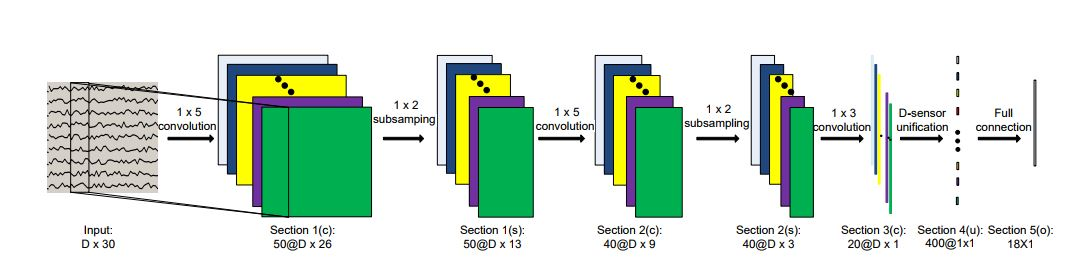
\includegraphics[width=10cm]{./image/a1} 
		\label{fig:sensor}		
	\end{center}
 \end{figure}

The CNN model includes convolution, subsampling, unification and output operations layers. This model also include one Data normalization layer. The activation function is ReLU (Rectified Linear Unit) function. 

\item The CNN model illustrated a higher accuracy on the gesture classification than other models [1].

\item \tiny [1]{JB. Yang \textit{et al}, Deep Convolutional Neural Networks On Multichannel Time Series For Human Activity Recognition}
\end{itemize}

\end{frame}

\begin{frame}
\frametitle{Hybrid of Neural Networks and Hidden Markov Model}

\begin{itemize}
\item Hybrid of Deep Neural Networks and Hidden Markov 

 \begin{figure}[htbp] 
	
	\begin{center}
		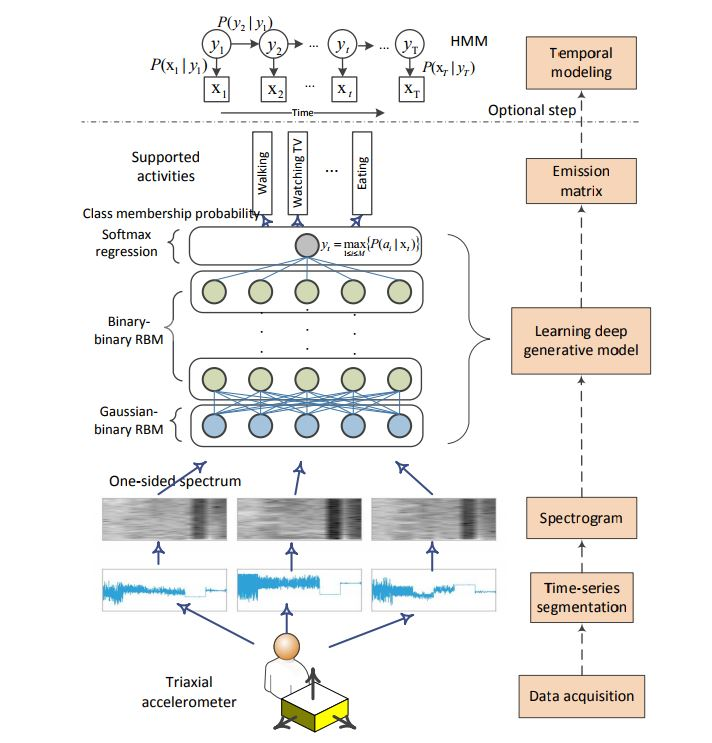
\includegraphics[width=6cm]{./image/a2} 	
	\end{center}
\end{figure}

\end{itemize}

\end{frame}

\begin{frame}
\frametitle{Hybrid of Neural Networks and Hidden Markov Model}
Step by Step Process
\begin{itemize}
\item[(1)] Takes triaxial acceleration time series 
\item[(2)] Extracts the spectrogram of windowed excerpts (from time domain to frequency domain) 
\item[(3)] Computes intrinsic features using a deep
generative model (Restricted Boltzman Machine (RBM), softmax regression)
\item[(4)] Recognizes the underlying
human activities by finding the posterior probability distribution (Hidden Markov Model)

\end{itemize}

Results: Approximately $3.5\%$ increase in the accuracy

\vspace{2em}
\scriptsize [2] Reference M.A Alsheikh \textit{et al} Reference: Deep Activity Recognition Models with Triaxial Accelerometers 

\end{frame}


\begin{frame}
\frametitle{CNN and LSTM Recurrent Neural Network}

The data format of the accelerometer and gyroscope data are both 3-dimensional and the the Conventional Deep Convolutional Neural Network can also be applied to the Gyroscope dataset.

\begin{itemize}
\item Process flowchart

 \begin{figure}[htbp] 
	
	\begin{center}
		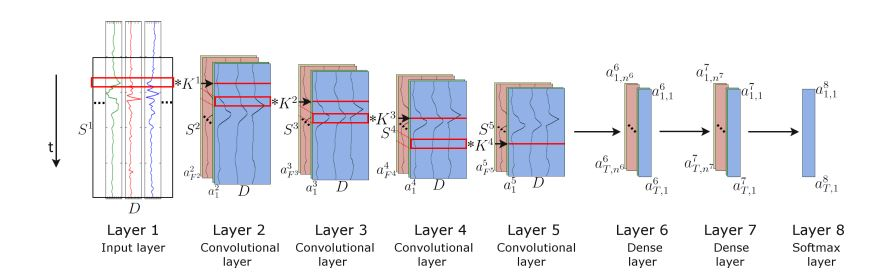
\includegraphics[width=7cm]{./image/g1} 	
	\end{center}
\end{figure}

\item This model is actually a cohesion of the CNN and LSTM (Long Short-term Memory) Recurrent Neural Network. 
\end{itemize}

\scriptsize References

\tiny [3] F.J. Ordonez \textit{et al.}, Deep Convolutional and LSTM Recurrent Neural Networks for Multimodal Wearable Activity Recognition, 2015

\tiny [4] S.C Yao \textit{et al.}, DeepSense: A Unified Deep Learning Framework for Time-Series Mobile Sensing Data Processing, 2017


\end{frame}

\begin{frame}
\frametitle{Useful Dataset Links}

\begin{itemize}
\item WISDM: Wireless Sensor Data Mining
\url{http://www.cis.fordham.edu/wisdm/dataset.php}

This website provide some dataset and the basic human body movement classifications are given. 

\item UCI Machine Learning Repository

This dataset is the Accelerometer and gyroscope data. Some basic body motion classifications are given. 

\url{https://archive.ics.uci.edu/ml/datasets/human+activity+recognition+using+smartphones}

\end{itemize}
\end{frame}

\begin{frame}
\frametitle{Week 1 Summary}

\begin{itemize}
\item The single Deep Learning Model, CNN and LSTM RNN can have good performance on data classification.

\item Cohesion of different models may increase the performance.

\item Sensor fusion is a common method of data pre-processing for the training of the Accelerometer and Gyroscope dataset. 
\end{itemize}

\end{frame}



\end{document}